\documentclass[../main.tex]{subfiles}
\begin{document}
\section{Approach} \label{sec:approach}

\subsection{Implementation and Software}

\subsubsection{Software}

The initial part of this master thesis was first to reimplement the TabNet architecture based on the original paper as described in section \ref{ssec:tabnet}. The original authors released a public available version, but not parameterize-able and using an outdated autograd backend (Tensorflow v1 \cite{tensorflow2015-whitepaper}). Additionally the implementation was mainly focused on the Covertype dataset \cite{noauthor_google-researchtabnet_nodate}. Even though other reimplementations of TabNet can be found it was decided to reimplement the original TabNet architecture to get better insight and being more flexible adding additional features and debugging options. 
\newline

A recent version of Pytorch \cite{NEURIPS2019_9015} is used as a autograd backend for the core TabNet components. Additionally Pytorch-Lighting (PL) \cite{falcon2019pytorch} was used as a wrapper for handling training loops, better logging capabilities and callbacks such as early stopping and checkpointing. PL also allows for more easy GPU utilization including multi GPU training and distributed GPU training over many machines. DL baselines for experiments were also implemented using Pytorch and PL. For random forests the scikit-learn \cite{scikit-learn} framework was used and as gradient boosting decision tree implementation XGBoost \cite{chen_xgboost_2016}.
\newline

The open source ML lifecycle stack MLflow \cite{noauthor_mlflow_nodate} was used for experiment tracking including metric and parameter tracking. It was self hosted using a S3\footnote{Simple Storage Service - object storage over a web service - first introduced by Amazon in 2006 \cite{noauthor_amazon_2021}} compatible backend storage for artifact storing like model checkpoints and plots. Details of the self hosted experiment setup can be found in \cite{clemens_kriechbaumer_clemens33mlflow_2021}. 

\subsubsection{Hyperparameters Search} \label{sssec:hyperparameters_search}

For hyperparameters search Optuna \cite{optuna_2019} and the Ax \cite{noauthor_ax_nodate} framework have been used. The goal of the hyperparameters search is to find the optimal set of hyperparameters to achieve the best result of an underlying unknown objective function, in this case a ML model. Iteratively a set of hyperparameters are chosen and used to train the underlying model resulting in a measurable result or metric. To try and compare all possible combinations of hyperparameters doing grid search is usually not feasible. Therefore usually random hyperparameters search or other methods like Bayesian optimization is utilized. 
\newline

Both mentioned frameworks are open source Bayesian hyperparameters optimization tools which iteratively update a prior belief about the impact of hyperparameters to a functions output or metric, in this case a ML model. Goal is to get a better posterior understanding about their relationship. First a number of initial runs, using randomly sampled hyperparameter sets, are used to build up a surrogate function describing the prior knowledge about the relationship between hyperparameters and function (ML model) outputs. This surrogate function or Gaussian process is a joint distribution of random variables, in this case hyperparameters which follows a multivariate normal distribution. Using the surrogate function an acquisition function is used to determine which hyperparameter set to use next. This is done by sampling from the surrogate function either by choosing a point of highest probability of improving (\acs{poi}) or by choosing the point with highest expected improvement (\acs{ei}) \cite{noauthor_exploring_nodate}. 

This iteratively process by choosing a new set of hyperparameters using the acquisition function and updating the surrogate function based on the results is repeated a predefined number of times or runs. Within each experiment in this work the hyperparameter search space as well as the number of total runs to find the optimal hyperparameters is described.

\subsubsection{Optimizer and Schedulers}

For DL parameter optimization algorithm for gradient descent as described in section \ref{sssec:dl} the variants Adam \cite{kingma_adam_2017} and AdamW \cite{loshchilov_decoupled_2019} were used. For learning rate schedulers a linear scheduler with warmup or an exponential decaying one were applied. After each parameter update or training step the learning rate is updated. For a linear scheduler with warmup this can be described using learning rate $\eta$ at given training step $s$ training for $N_{steps}$ with $N_{warmup}$ warm up steps as follows:

\begin{equation}
	\eta_{new}=
    \begin{cases}
        \eta \cdot \frac{s}{N_{warmup}},& \text{if } s<N_{warmup} \\
        \eta \cdot \frac{N_{steps} - s}{N_{steps} - N_{warmup}},& \text{otherwise } \\
    \end{cases}	
\end{equation}

An simple exponential decaying scheduler with its settings decaying rate $\beta$ and decaying step $\lambda$ is given by:

\begin{equation}
	\eta_{new}=\eta \cdot \beta^{\frac{s}{\lambda})}
\end{equation}

Additionally the following figure \ref{fig:scheduler_linear_exponential} plots the behavior of the learning rate using different settings.

\begin{figure}[H]
    \centering
    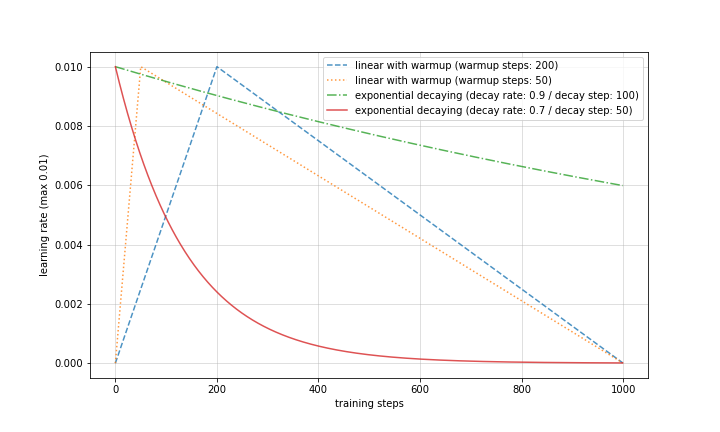
\includegraphics[width=0.7\textwidth]{scheduler_linear_exponential}    
    \caption{Linear and exponential decaying learning rate scheduler}
    \label{fig:scheduler_linear_exponential}
\end{figure}

The authors of TabNet used Adam optimizer with an exponential decaying learning rate scheduler in all of their experiments. Further within their release code repository \cite{noauthor_google-researchtabnet_nodate} gradient clipping was applied. Gradient clipping is a technique to manually clip gradients if the norm or values of the gradient are above a defined threshold to mitigate the exploding gradient issue and numerical problems. The reimplementation of TabNet within this master thesis has the option to apply gradient clipping. The exact setup (optimizer, scheduler and gradient clipping) is described within each of the experiments. 

\subsubsection{Infrastructure and Hardware} \label{sssec:infrastructure_and_hardware}

All experience were performed on a regular desktop computer with Ubuntu 20.04 as operating system powered by an AMD Ryzen 3700X with 64GB memory. Two GPUs, NVIDIA GTX 1070 with 8GB memory and NVIDIA GTX 1080 Ti with 11GB were used in a single node multi GPU setup for training the various DL models. Depending on the hyperparameters TabNet can be considered a compact DL architecture with usually between a few 100K parameters to maximum of single digit million parameters. Therefore it is feasible to train a TabNet based model from scratch without any hardware barrier and can not be compared to architectures like transformers with tens of millions of parameters.
\newline

For source control Git with GitHub\footnote{\url{https://github.com/}} as backend was used. The TabNet reimplementation including all source codes including the experiments is available within a public repository \cite{kriechbaumer_clemens33thesis-tex_nodate}. The experiment metrics including parameters used are available under a public available domain\footnote{All experiments are available at \url{mlflow.kriechbaumer.at} for atleast 1 year after release of this work - later on experiments can be made available after contacting the author} for at least 1 year after release of this work. The self hosted environment is based on MLFlow and described in \cite{kriechbaumer_master_nodate}.
For testing the framework pytest \cite{krekel_pytest_2004} was used. All core components of the TabNet reimplementation, this includes the individual components like attentive transformer, feature, decision step or sparsemax implementation were tested including gradient checking which especially important for the sparsemax part. 

\subsubsection{TabNet Implementation Details} \label{sssec:tabnet_implementation_details}

Based on described architecture in section \ref{ssec:tabnet} the TabNet architecture was implemented. Due to the novel character in following the most relevant and untypical hyperparameters are explained. Some of them are added or adapted compared to the authors TabNet implementation \cite{noauthor_google-researchtabnet_nodate} and offer an additional flexibility and options.

\begin{itemize}
	\item \textbf{Input size} - refers to input feature dimensions
	\item \textbf{Feature size} - refers to internal hidden size for feature representation. The decision size $N_d$ and the information output size $N_a$ together are the feature size.
	\item \textbf{Decision size} - this is TabNet output size.
	\item \textbf{Number layers} - how many layers (\acs{fc}, \acs{bn} and GLU) each decision step within the feature transformer is using.
	\item \textbf{Number shared layers} - how many of those layers are shared between the decision steps. This significantly reduces the models trainable parameter count. If there are shared layers they are first run through within the feature transformer.
	\item \textbf{Number steps} - how many decision steps are used in the model.
	\item \textbf{Gamma, $\gamma$} - this is the relaxation parameter which controls if an individual feature is more likely used in multiple steps or not. If$\gamma$ is close to 1 reusing of features is more strict if $\gamma$ gets larger reusing is more relaxed. Details can be found in equation \ref{eq:gamma}.
	\item \textbf{Relaxation type} - beside the value for $\gamma$ this additional hyperparameter allows additional control of the relaxation hyperparameter.

	\begin{itemize}
		\item \emph{$\gamma$ fixed} - this is the default value, handling gamma as a hyperparameter in the same way as the authors TabNet implementation.
		\item \emph{$\gamma$ not applied} - Previous feature selection masks are not considered and the equation \ref{eq:gamma} is not applied.
		\item \emph{$\gamma$ shared trainable} - converts $\gamma$ from a hyperparameter to one trainable parameter shared across all decision steps. 
		\item \emph{$\gamma$ trainable} - converts $\gamma$ from a hyperparameter to a trainable parameter per decision step. 
	\end{itemize}

	\item \textbf{Attentive type} - The authors TabNet implementation used Sparsemax exclusively for feature selection. This reimplementation allows to use alternative attentive methods. Those alternative methods include the $\alpha$-entmax function with arbitrary alphas as described in section \ref{sssec:sparsemax} using the $\alpha$-entmax authors implementation as backend \cite{noauthor_entmax_2021}.

	\begin{itemize}
		\item \emph{Sparsemax} - default value and using sparsemax for feature selection.		
		\item \emph{Entmax1.5} - uses the numerically optimized version of $\alpha$-entmax when $\alpha=1.5$.
		\item \emph{$\alpha$-entmax} - uses $\alpha$-entmax with an arbitrary value for $\alpha>1$
		\item \emph{$\alpha$-entmax - $\alpha$ shared trainable} - uses $\alpha$-entmax but $\alpha$ itself becomes a trainable parameter shared across all decision steps.
		\item \emph{$\alpha$-entmax - $\alpha$ trainable} - uses $\alpha$-entmax but $\alpha$ itself becomes a trainable parameter per decision step.				
	\end{itemize}
	
	\item \textbf{Epsilon $\epsilon$} - a small value for numerical stability when calculating the sparsity regularization term in equation \ref{eq:sparsity_regularization}.

	\item \textbf{$\lambda$ sparse} - Controls the amount of sparsity regularization as described in equation \ref{eq:lambda_sparse}.

	\item \textbf{Momentum} - the momentum term for calculating the running average for the mean $\mu$ and variance $\sigma$ statistics in all batch norm used in the model.

	\item \textbf{Virtual batch size} - This describes the chunk size for ghost batch norm as described in section \ref{sssec:feature_transformer}. Additionally if the value is not given no batch norm is applied within the feature and attentive transformer of the TabNet model.

	\item \textbf{Normalize input} - Controls if batch norm is applied onto the raw input features or not. The original paper describes to use raw (not normalized)features for the TabNet model, but first apply batch norm. Note for the input batch norm default batch norm (not ghost batch norm) is used. 
\end{itemize}

The amount of hyperparameters also emphasize the novel character of the TabNet architecture but is especially relevant and potential problematic for hyperparameter search.

\subsubsection{TabNet Metrics and Logging}

The TabNet reimplementation allows for logging of the average sparsity, or one average how many individual feature dimension over a given dataset have not been considered. Given batch size $B$ and feature dimension $N$ using the Kronecker delta $\delta$ and the aggregated feature selection mask $\mathbf{M} \in \mathbb{R}^{B \times N}$ this is calculated as follows:

\begin{equation} \label{eq:sparsity}
	m_{sparsity}=\frac{1}{B \cdot N}\sum_{b=1}^{B} \sum_{i=1}^{N} \delta_{\mathbf{M}_{bi}, 0}
\end{equation}

The sparsity metric $m_{sparsity}$ can be calculated on the overall level using the aggregated feature selection masks, as described in equation \ref{eq:aggregated_mask}, or using individual feature selection mask per decision step.

Other metrics used were accuracy and the area under the receiver operator characteristic (\acs{auroc}) curve. 

\subsubsection{Verification}

Before any experiments within the drug discovery domain were performed the reimplementation was verified based on the achieved results using the Covertype dataset, refer to section \ref{ssec:covertype}. As all relevant hyperparameter were known including random seeds and dataset splits this resulted in the following setup. 

\begin{itemize}
	\item \emph{Hyperparameters}: Number of decision steps $N_{steps}=5$, hidden feature size $N=128$, TabNet decision output size $N_d=64$, relaxation parameter gamma $\gamma=1.5$, regularization parameter $\lambda_{sparse}=0.0001$, batch norm momentum $m_B=0.3$ with virtual batch size $B_V=512$ for ghost batch norm, training batch size $B=16384$, number shared layers $2$ and number of individual layers $2$
	\item \emph{Optimizer and Scheduler}: Adam with learning rate $\eta=0.02$ with exponential decaying learning rate scheduler using rate $\beta=0.95$ decaying every $500$ steps was used. Gradient clipping based on absolute gradient value above $2000$ was performed.
	\item \emph{Data preprocessing}: The same splits as described in section \ref{ssec:covertype} were used. Per categorical dimension (44 binary feature dimensions) 1 dimensional embeddings are trained.	
\end{itemize}

Using this setup the model was trained about 3 hours with described infrastructure, refer to section \ref{sssec:infrastructure_and_hardware}.  The results of the reimplementation "my TabNet" compared with the TabNet authors results can be seen in following table \ref{tbl:tabnet_verified}. The TabNet reimplementation achieves similar results than the TabNet authors reported results. The minor differences were not further analyzed but could be explained in the more than 4 times higher maximum training steps, potential numerical differences resulting from varying initialization strategies used, as well as different and variations in software packages. 

\begin{table}[H]
    \centering
    \begin{tabular}{ |c|c|} 
        \hline
        \rowcolor{lightgray} \textbf{Model} & \textbf{Test accuracy (\%)} \\
        \hline
        \emph{XGBoost} &  89.34 \\
        \emph{LightGBM} &  89.28 \\
        \emph{CatBoost} &  85.14 \\
        \emph{AutoML Tables} &  94.95 \\
        \emph{TabNet} \tablefootnote{ about 130K training steps} &  96.99 \\
        \hline
        \textbf{my TabNet} \tablefootnote{ about 30K training steps - for all details refer to \url{https://mlflow.kriechbaumer.at/#/experiments/39/runs/fb30421c0cb34cdda54a7d961a09c7ad}} & 96.38 \\
     \hline
    \end{tabular}
    \caption{TabNet reimplementation verification results}
 	\label{tbl:tabnet_verified} 	
\end{table}

Furthermore the effect of using a different attentive strategies using the Covertype dataset was briefly explored. Within the following table \ref{tbl:tabnet_attentive_strategies} the achieved accuracy as well as the average sparsity as explained in equation \ref{eq:sparsity} is visible. Achieved values are not representative, due to no hyperparameter tuning or repeated experiments with different random seeds and splits. Those runs are a teaser and give a better intuition especially about the sparsity behavior of different attentive types. 

\begin{table}[H]
    \centering
    \begin{tabular}{ |c|c|c| } 
        \hline
        \rowcolor{lightgray} \textbf{Model} & \textbf{Test accuracy (\%)} & \textbf{Sparsity} (\%) \\
        \hline
        \textbf{TabNet} &  96.38 & 75.80 \\
        \emph{TabNet ($\gamma$ shared trainable}) & 96.59 & 32.03 \\
        \emph{TabNet ($\alpha=3.0$-entmax}) &  94.28 & 86.34 \\
        \emph{TabNet ($\alpha=1.5$-entmax}) &  96.34 & 27.10 \\
        \emph{TabNet (Softmax)} &  96.07 & 0 \\        
     \hline
    \end{tabular}
    \caption{TabNet reimplementation using different attentive strategies}
 	\label{tbl:tabnet_attentive_strategies} 	
\end{table}

In addition in figure \ref{fig:covtype_training_behavior} the training behavior of TabNet on the Covertype dataset is shown for different attentive strategies is illustrated. On the y axis the corresponding values for the TabNet loss term (cross entropy loss plus sparsity regularization), the achieved accuracy and the sparsity as given in equation \ref{eq:sparsity} are shown. Data was collected on the validation Covertype dataset split during training. 
Additionally experiments or different effects of attentive strategies have not been further explored within this master thesis.

\begin{figure}[H]
    \centering
    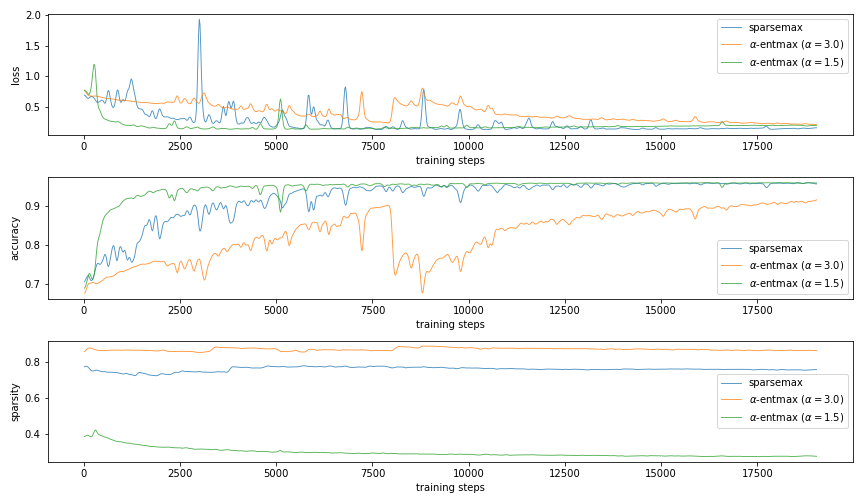
\includegraphics[width=1.0\textwidth]{covtype_training_behavior}        
    \caption{Training behavior of TabNet on the Covtype dataset using different attentive strategies}
    \label{fig:covtype_training_behavior}
\end{figure}

\subsubsection{Interpretability and Plotting} \label{sssec:tabnet_implementation_interpretability}

The TabNet reimplementation allows for plotting of the feature selection masks as a heatmap, either using aggregated $M_{agg}$ or individual $M^{[l]}$ feature selection mask. In figure \ref{fig:covtype_aggregated_mask} an example of the plotted $M_{agg}$ for 25 samples of the Covertype test dataset using the trained TabNet model with attentive type sparsemax is shown. The corresponding labels per sample are displayed on the y axis and on the x axis the feature dimensions and names is given. In figure \ref{fig:covtype_masks_overview} all individual $M^{[l]}$ for all the 5 decision steps on the same 25 samples are visualized. 

\begin{figure}[H]
    \centering
    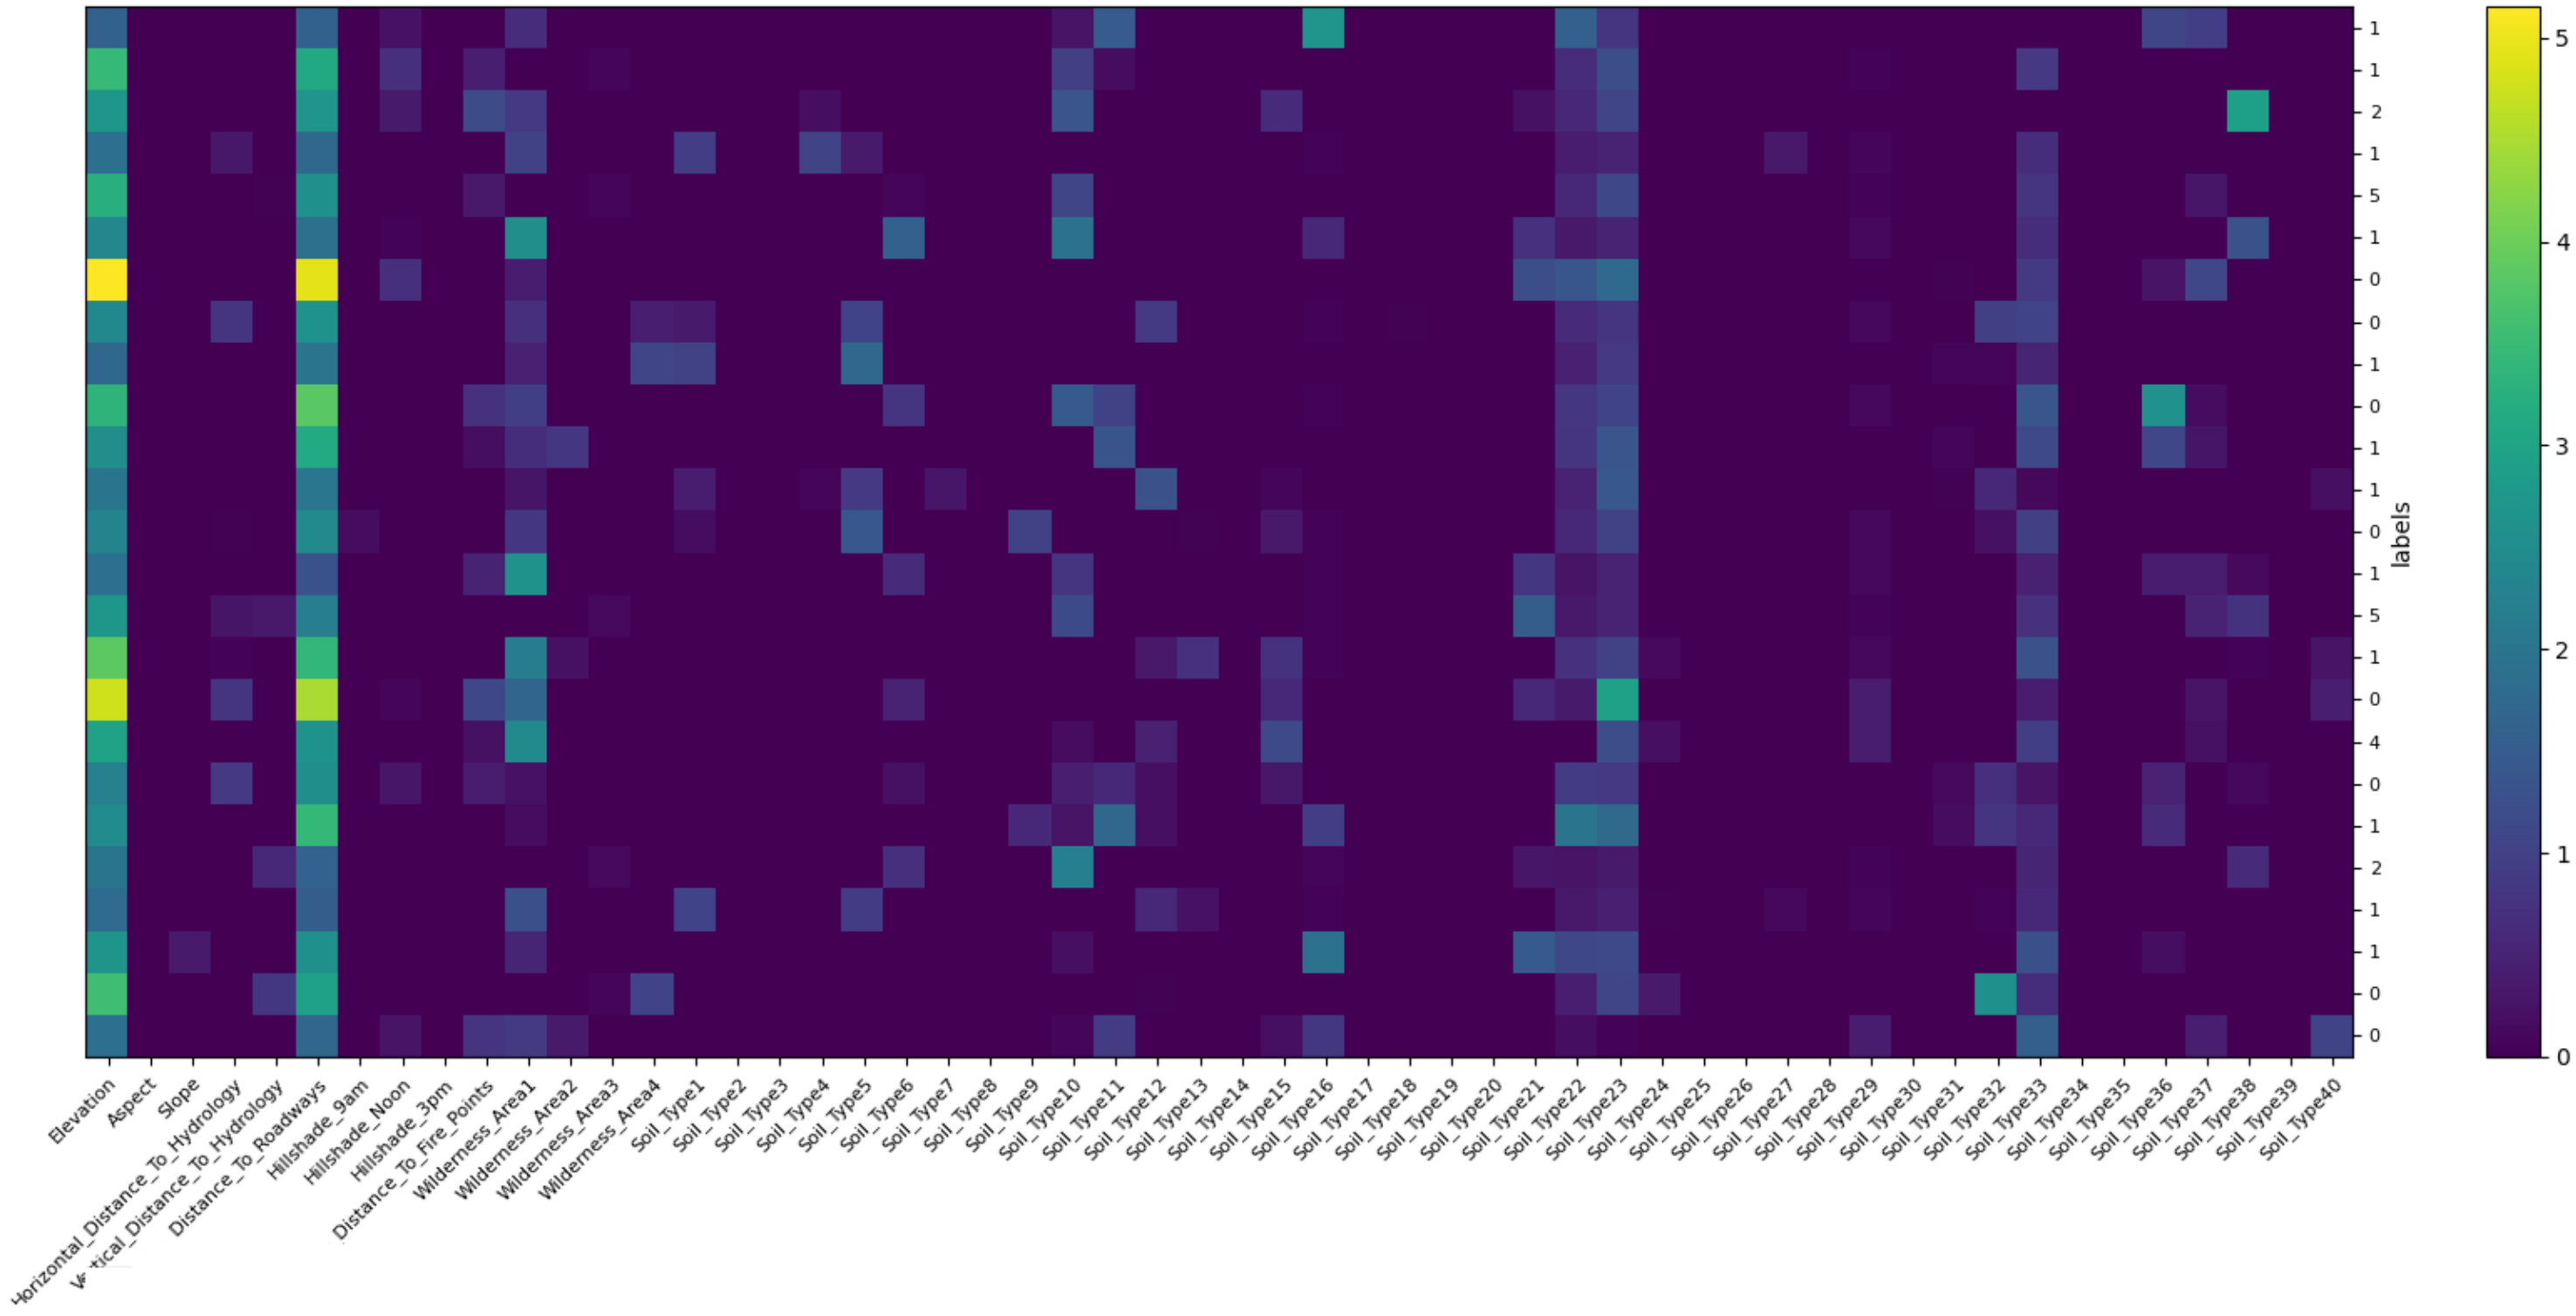
\includegraphics[width=1.0\textwidth]{covtype_aggregated_mask}        
    \caption{Aggregated mask $M_{agg}$ visualized on sample entries of the Covertype test dataset}
    \label{fig:covtype_aggregated_mask}
\end{figure}

\begin{figure}[H]
    \centering
    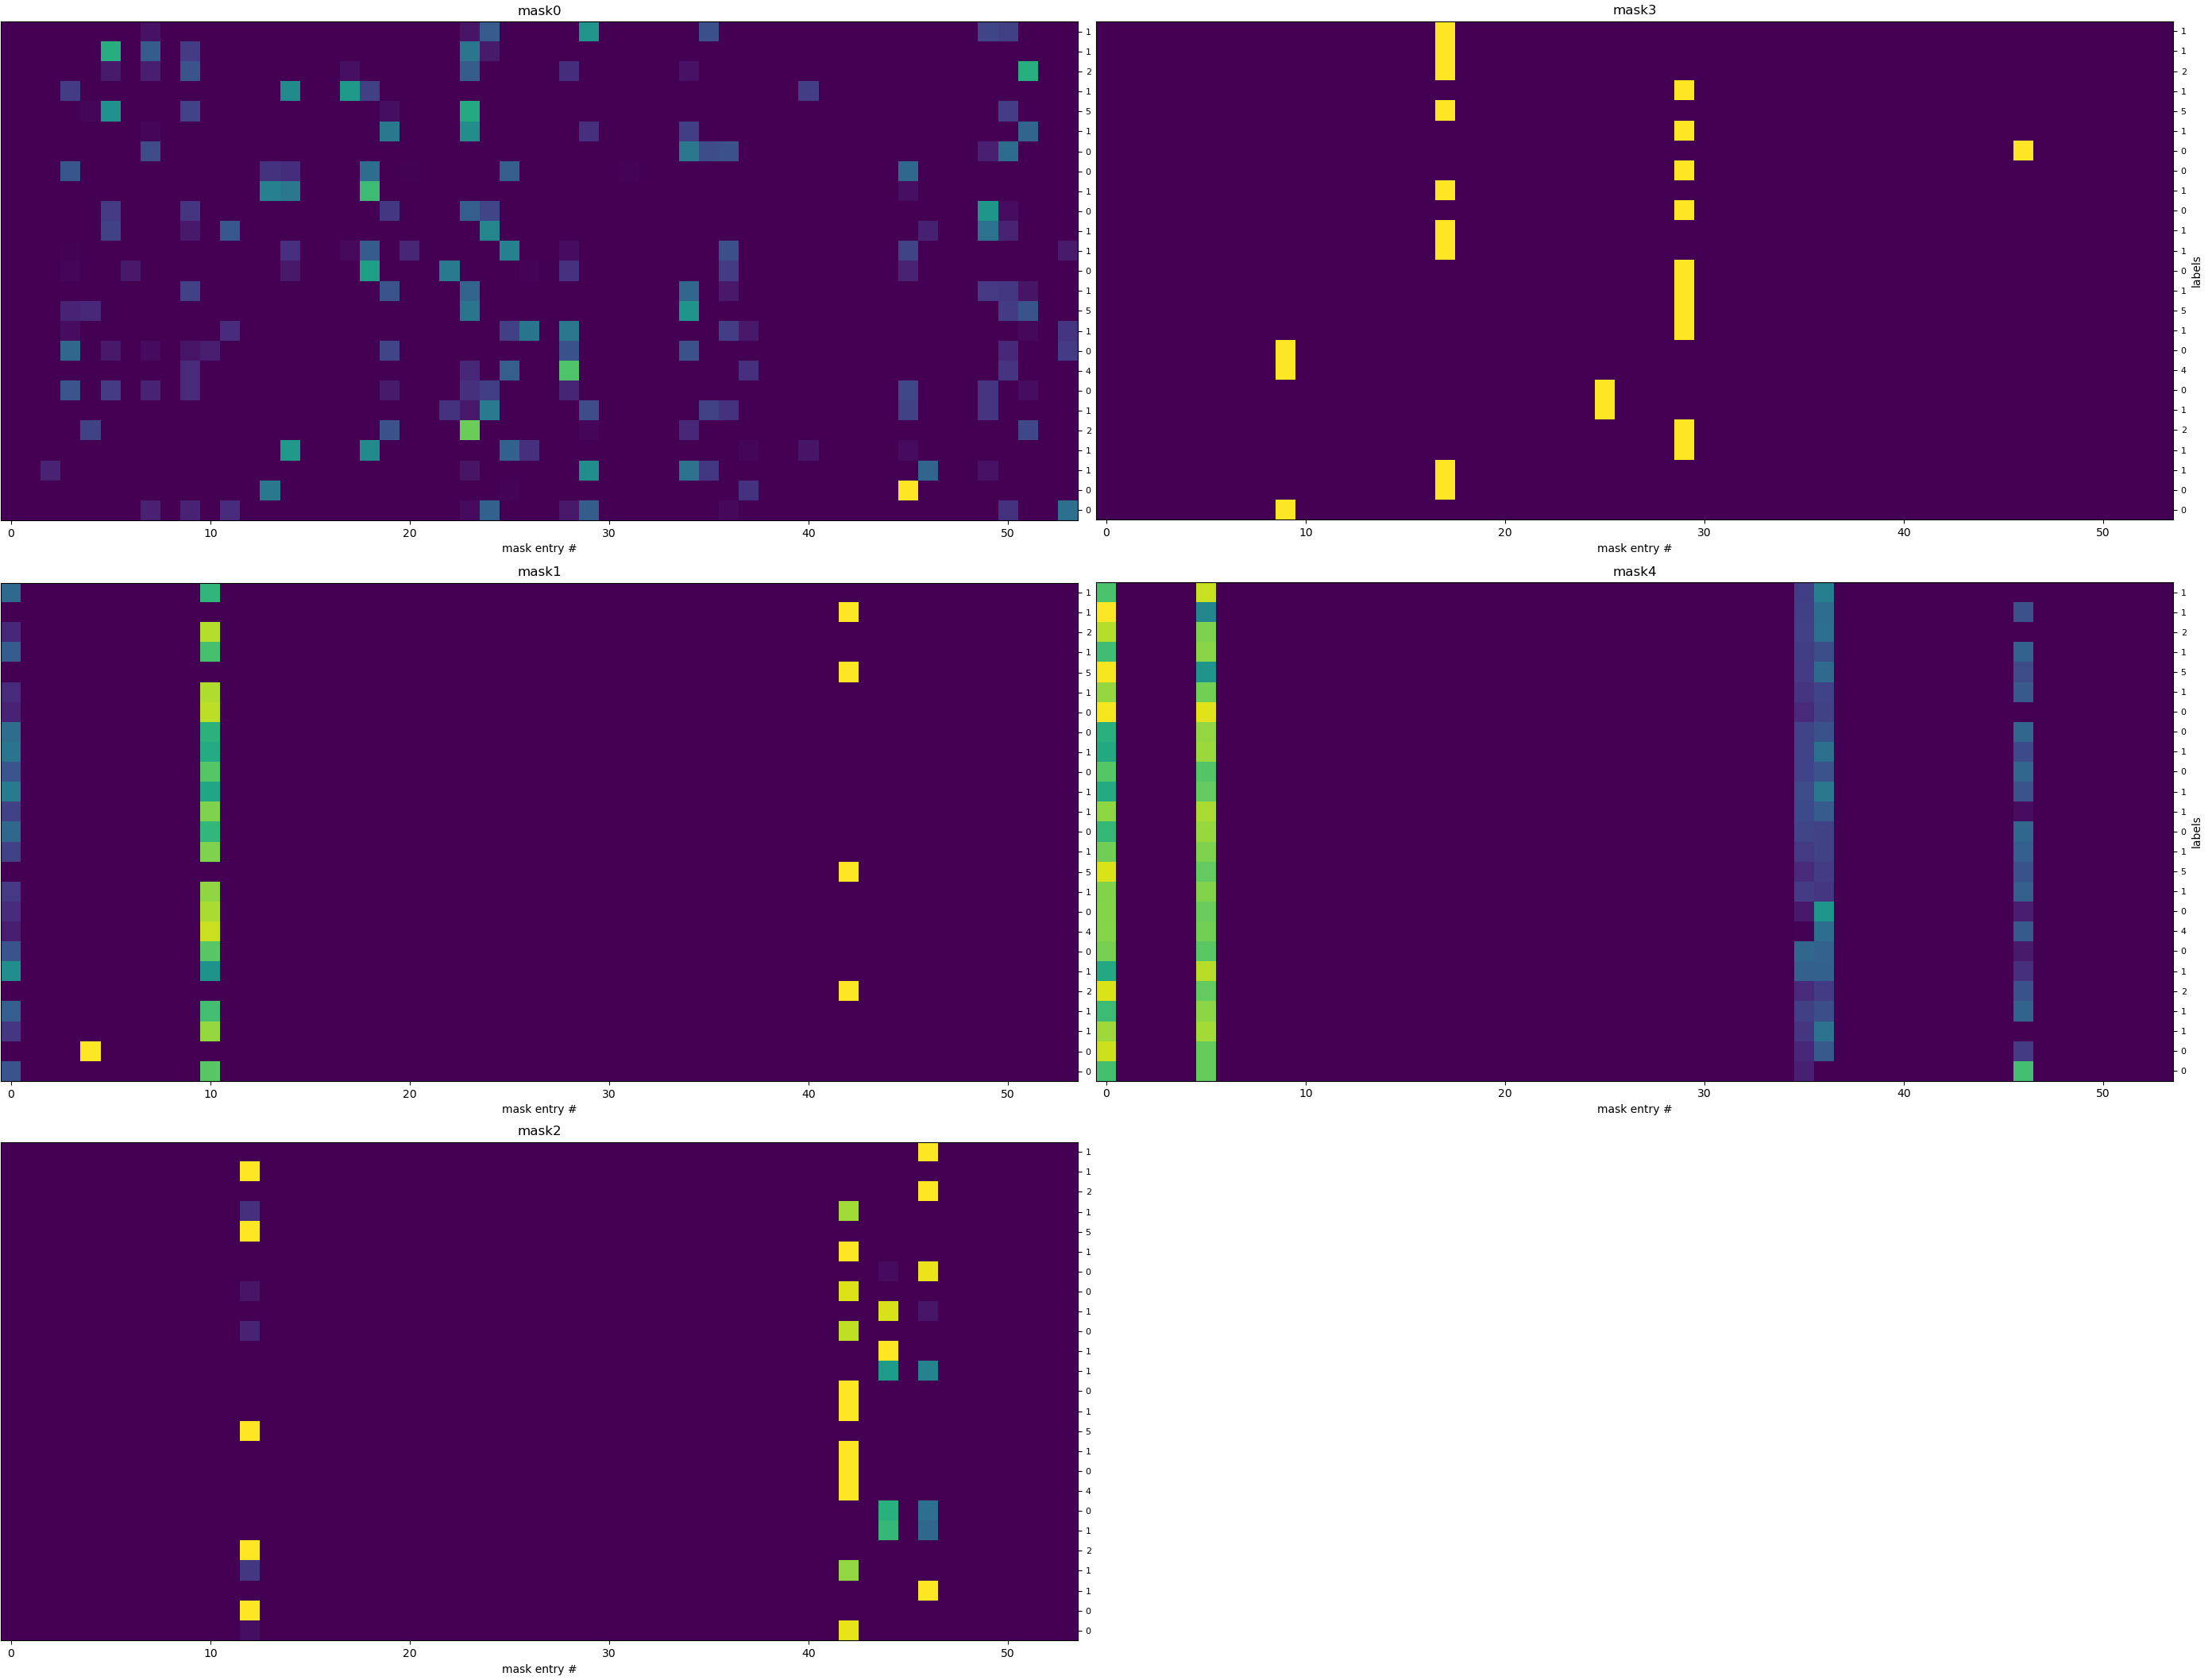
\includegraphics[width=1.0\textwidth]{covtype_masks_overview}        
    \caption{Individual masks on samples of the Covertype test dataset}
    \label{fig:covtype_masks_overview}
\end{figure}

By using the visualized feature selection mask it can be seen that some features, like for Covertype "Elevation" or "Distance to Roadways" seams to be important for all individual samples. When looking at the overview of all masks (figure \ref{fig:covtype_masks_overview}) it can be seen that within the TabNet architectures individual decision steps specialize on different features. 
Using all entries in a dataset and calculate the mean and standard deviation for each feature dimension within the $\mathbf{M_{agg}}$ the average importance and ranking of each feature can be determined. An example is shown in figure \ref{fig:covtype_feature_ranking} for which on the left the average feature ranking using sparsemax and on the right using $\alpha$-entmax with $\alpha=3.0$ is presented. The concrete ranking with "Elevation" being the most important feature on average confirms the first impression while only looking at 25 samples as given in figure \ref{fig:covtype_aggregated_mask}. Furthermore it shall be noted that the $\alpha$-entmax with $\alpha=3.0$ variant is much more sparse. It only uses 20 feature dimensions, meaning considering all test samples only 20 features were considered to be relevant. 

\begin{figure}[H]
    \centering
    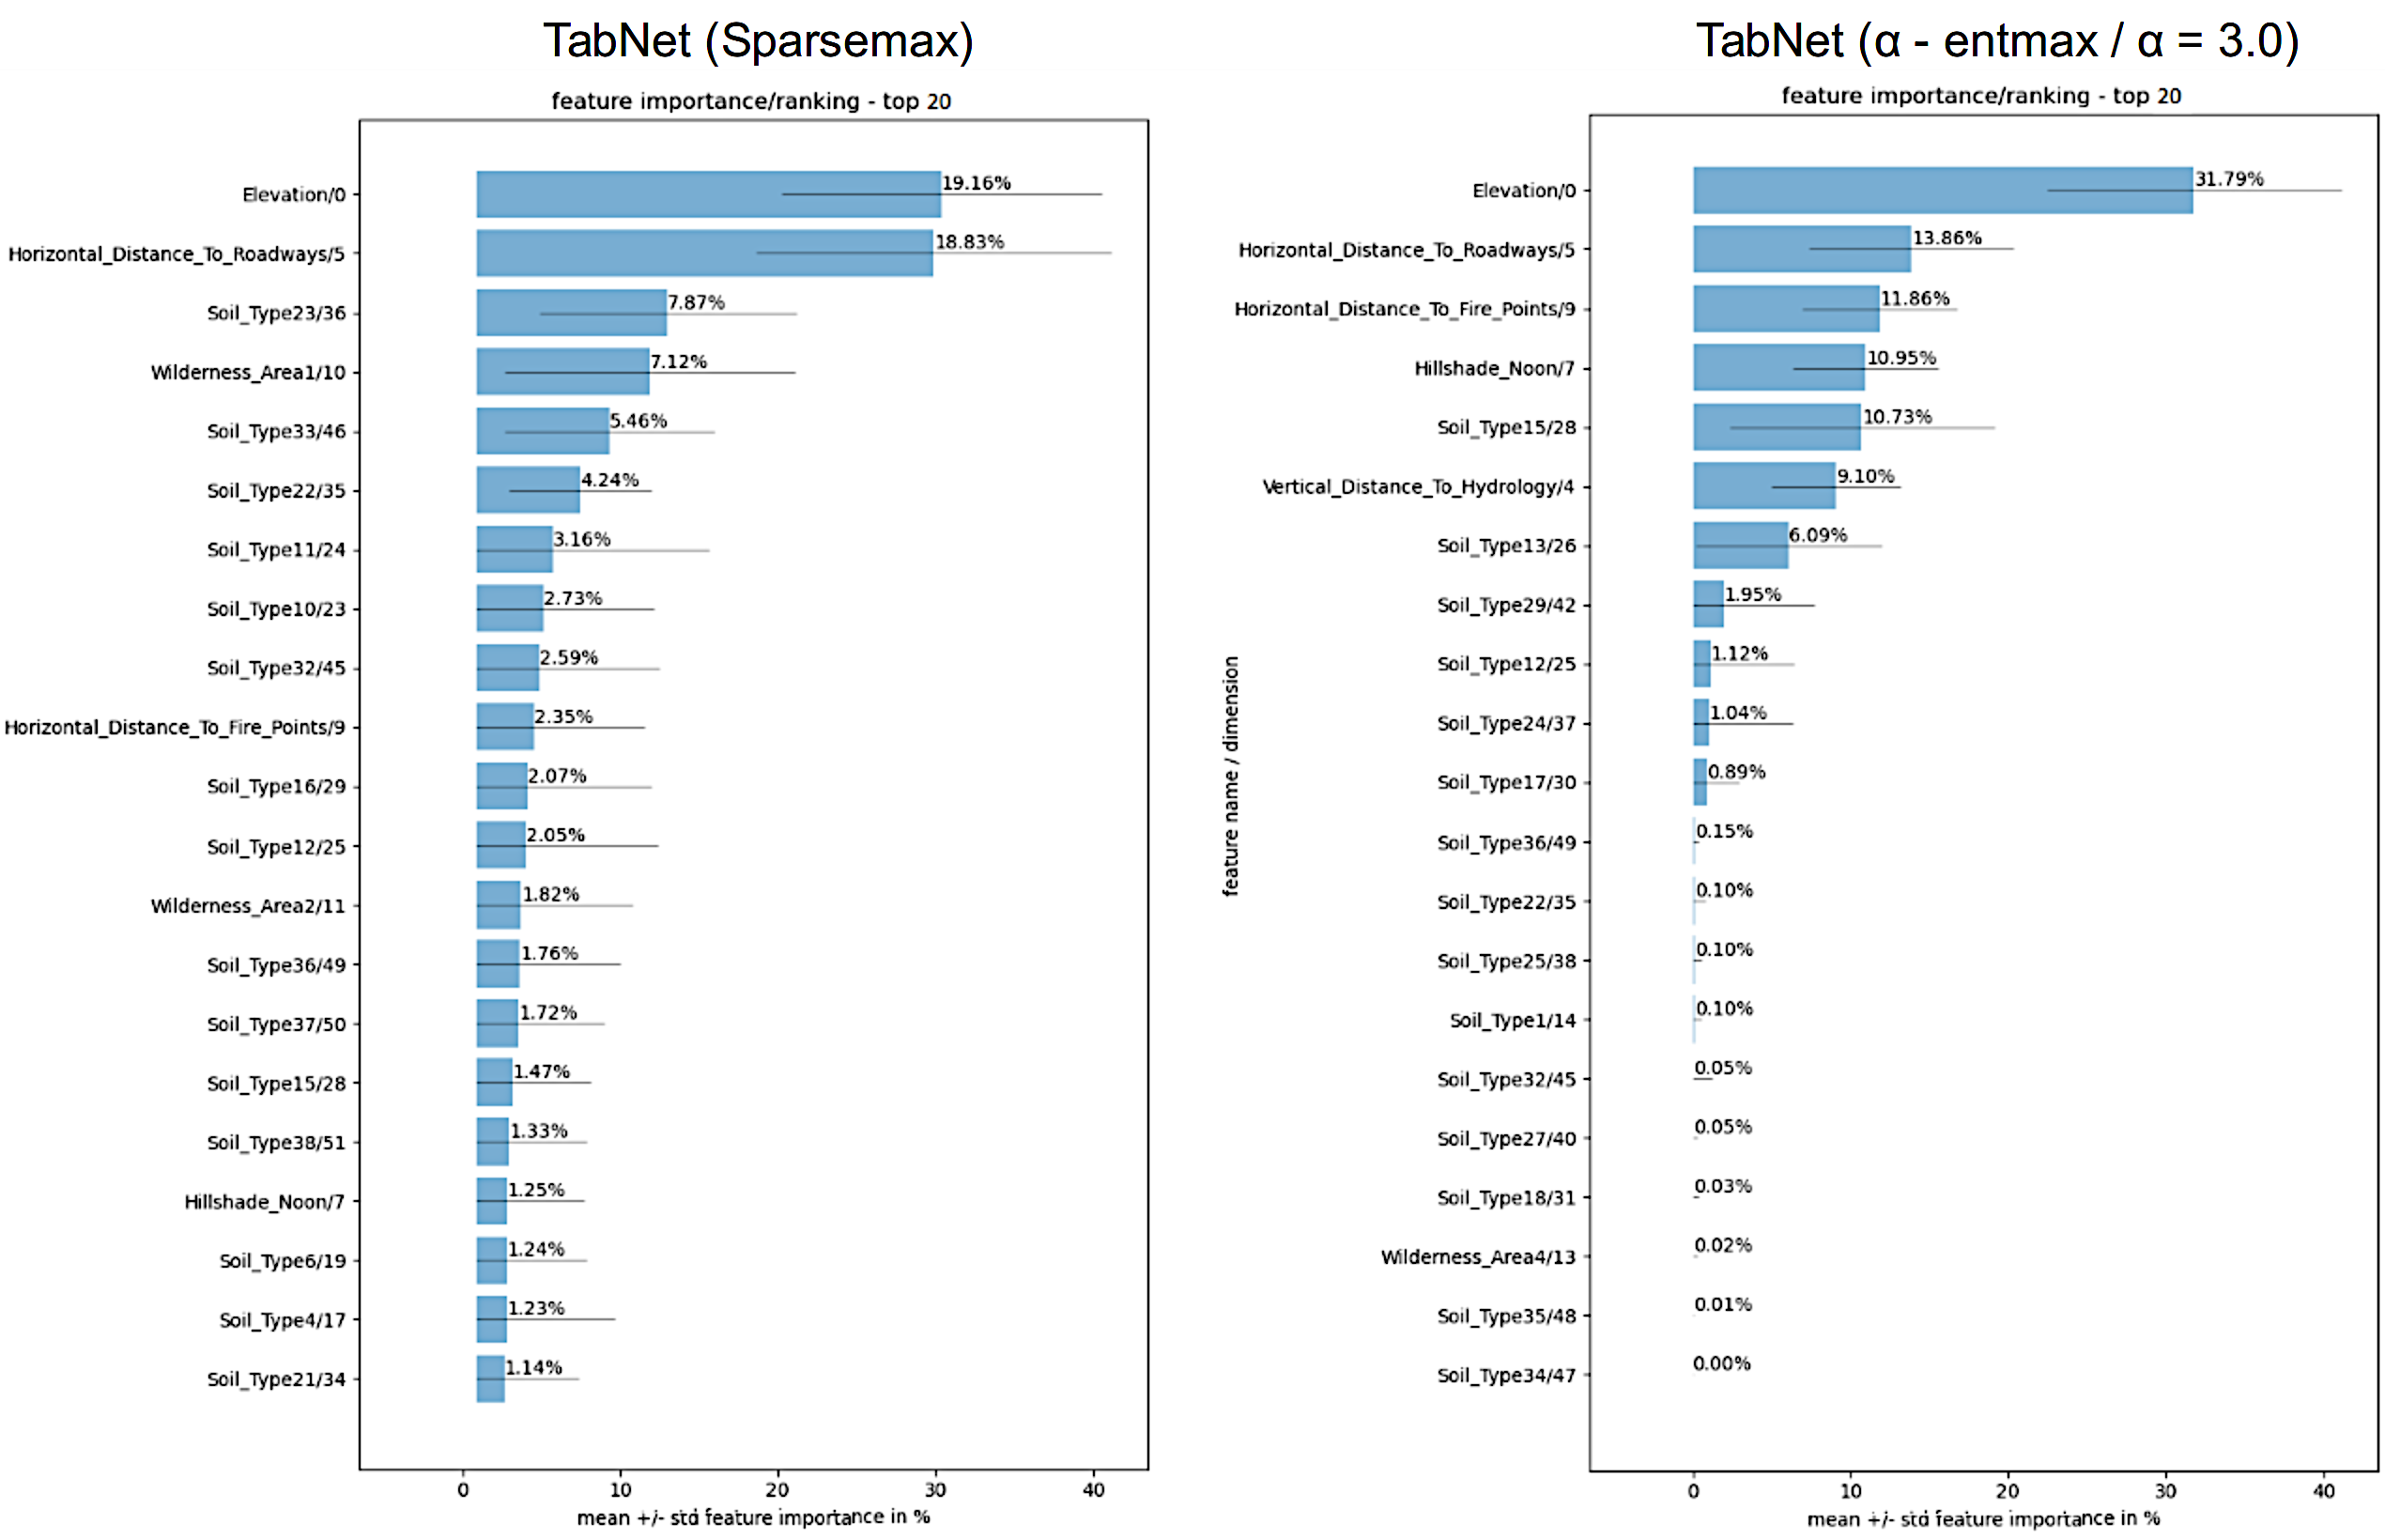
\includegraphics[width=1.0\textwidth]{covtype_feature_ranking}        
    \caption{Average feature importance ranking of the Covertype test dataset using two different attentive types}
    \label{fig:covtype_feature_ranking}
\end{figure}

\newpage
    
\end{document}